\documentclass{article}
\usepackage[utf8]{inputenc}

\title{MI-PAA: Problém batohu}
\author{Josef Doležal}

\usepackage{natbib}
\usepackage[czech]{babel}
\usepackage{a4wide}
\usepackage{graphicx}

\begin{document}

\maketitle

\section{Úvod}
Problémem batohu se nazývá úloha, ve které je za úkol pro množinu $n$ předmětů a batoh o maximální nosnosti $m$ určit, jak předměty do batohu vložit tak, aby v součtu měly co největší hodnotu a zároveň nebyla překročena maximální nosnost batohu.

Vstupem je tedy seznam $n$ předmětů (dvojic váha-cena) a maximální nosnost batohu $m$.
Výstupem je v součtu nejvyšší možná cena předmětů, jejichž váha dohromady nepřekročí nosnost.

\section{Zadání úlohy}

\begin{enumerate}
    \item Naprogramujte řešení problému batohu hrubou silou (tj. exaktně). Na zkušebních datech pozorujte závislost výpočetního času na $n$.
    \item Naprogramujte řešení problému batohu heuristikou podle poměru cena/váha. Pozorujte:
    \begin{itemize}
        \item závislost výpočetního času na $n$. Grafy jsou vítány (i pro exaktní metodu).
        \item průměrnou a maximální relativní chybu (tj. zhoršení proti exaktní metodě) v závislosti na $n$.
    \end{itemize}
\end{enumerate}

\section{Možná řešení}

Zadaný problém je možné řešit více způsoby.
Implementačně nejjednodušším se jeví vyzkoušení všech možných kombinací (tzv. řešení hrubou silou).
Další možností je využití heuristik. Příkladem heuristik může být vkládání podle poměru cena/váha, vkládání nejlehčích předmětů nebo vkládání nejcennějších předmětů.

Využití heuristického algoritmu nemusí vždy dát správný výsledek, může ale nabídnout nižší časovou a/nebo paměťovou náročnost programu.

\section{Rámcový popis řešení}

Zadání úlohy specifikuje vyřešit problém pomocí hrubé síly a heuristikou podle poměru cena/váha.
Implementace problému je řešena pomocí programovacího jazyka Swift.

Program načte instance problému z referenčních vstupních souborů a dále referenční výstupy pro možnost ověření správnosti.

Předpokladem správné funkčnosti programu je, že referenční vstupy jsou seřazené stejným způsobem jako výstupy.
Na základě tohoto předpokladu program spáruje instanci problému s očekávaným řešením.

Pro každou instanci program vyřeší problém hrubou silou a výstup ověří vůči referenčnímu zadání.
Dále je problém vyřešen pomocí heuristiky.
Pro obě řešení program změří procesorový čas, který byl potřebný k získání výsledku.
Jako poslední krok vypočítá relativní odchylku řešení heuristikou od optimálního řešení.
Výsledky jsou poskytovány jako datový vstup pro program Gnuplot a \LaTeX{}.

Z důvodu automatického testování je program rozdělen do čtyř částí.
Tyto části jsou testovány pomocí jednotkových testů.
Správné propojení jednotlivých modulů je testováno až za běhu pomocí kontroly oproti referenčním výstupům.

\section{Popis algoritmu}

V této části rozebírám konkrétní implementaci jednotlivých řešení.
Součástí popisů jsou grafy, znázorňující časovou závislost na počtu předmětů.

\subsection*{Metoda hrubé síly}

Řešení touto metodou prochází všechny možné kombinace vložení předmětů.
Jedná se tedy problém průchodu všech podmnožin $n$ předmětů.

Celkový počet podmnožin množiny $n$ předmětů je $2^n$.
Program musí projít každou z těchto podmnožin (o nejvýše $n$ prvcích) a vypočítat její hodnotu jako součet cen předmětů.
Z tohoto důvodu je časová složitost $O(n \cdot 2^n)$.

\begin{figure}[h]
    \centering
    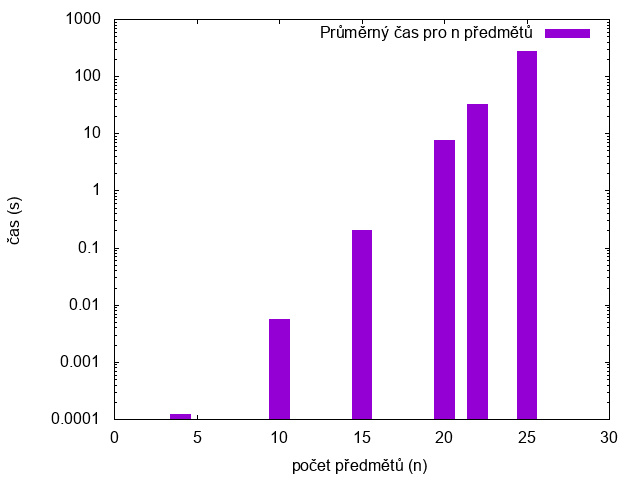
\includegraphics[width=0.8\textwidth]{all-cases-duration.png}
    \caption{Průměrný čas pro 50 instancí a $n$ předmětů}
    \label{fig:g1}
\end{figure}

Na obrázku \ref{fig:g1} je znázorněna časová náročnost této metody.
Časová náročnost byla měřena jako procesorový čas, který je potřebný k výpočtu jedné instance.
Graf znázorňuje průměrný čas pro 50 instancí řešeného problému.

Vzhledem k velkému rozptylu má graf na ose Y logaritmické měřítko.
Z grafu je patrný trend růstu času pro zvyšující se počet předmětů.
Růst přibližně odpovídá odhadu časové složitosti $O(2^n)$, tedy že s každým přidaným předmětem se čas přibližně zdvojnásobí.

Z důvodu velkého nárustu časové složitosti nebyl program testován na veškerých vstupech.
Pro vstupy o více než 25 předmětů se časová složitost blížila k době trvání jedné hodiny pro jednu instanci. 

\subsection*{Heuristika podle poměru cena/váha}

Implementace heuristiky je provedena ve třech krocích.
V prvním se provádí výpočet poměru cena/váha.
Následně jsou průměry sestupně seřazeny.
Po seřazení se prochází váhy a ceny předmětů od nejvyššího poměru tak dlouho, dokud v součtu nepřekročí maximální nosnost batohu.
Protože průchody polem předmětů mají lineární složitost, celková složitost se nejvíce odvíjí od složitosti řazení.

Standardní knihovna jazyka Swift využívá pro řazení Introsort\citep{swift-introsort}.
Tento algoritmus se skládá z QuickSort a HeapSort\citep{wiki-introsort} algoritmů.
Časová složitost tohoto řazení je v průměru $O(n \cdot \log n)$.

Celková složitost řešení jedné instance je $O(n + n \cdot \log n)$, ekvivalentně tedy $O(n \cdot \log n)$.

\begin{figure}[h]
    \centering
    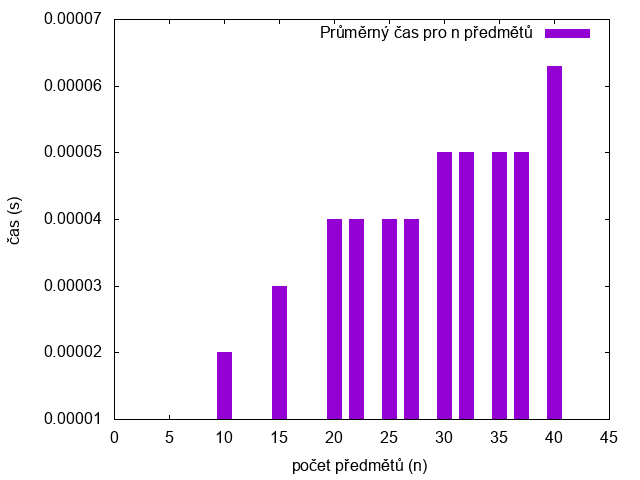
\includegraphics[width=0.8\textwidth]{heuristic-duration.png}
    \caption{Průměrný čas pro 50 instancí a $n$ předmětů}
    \label{fig:g2}
\end{figure}

Obrázek \ref{fig:g2} znázorňuje časovou složitost výpočtu za pomoci heuristiky.
Časová náročnost má pro rostoucí počet předmětů linární charakter.
Z grafu lze vyčíst, že časová náročnost je mnohem nižší než u exaktního výpočtu v předchozím případě.
To potvrzuje domněnku vyslovenou v úvodu zprávy o možných řešeních problému.
Oproti metodě hrubé síly ale nedává vždy správný výsledek a je tak nutné sledovat odchylky od očekávaných hodnot.
Více o odchylkach a chybách zmiňuji v další sekci.


\subsubsection*{Relativní chyba výpočtu}

Heuristické řešení problému vnáší do řešení možnost nepřesností a chyb.
Během měření výsledků metody cena/váha jsem počítal relativní a maximální odchylku od referečního výstupu.
Tabulka \ref{tab:approximation-error} znázorňuje průměrnou a maximální odchylku pro 50 instancí.

\begin{table}
\centering
    \begin{tabular}{ |r||r|r| } 
        \hline
        $n$ & Průměrná relativní chyba & Maximální relativní chyba \\
        \hline
        \hline
         4 & 2.17450811344437 & 36.3636363636364 \\
        10 & 1.28619858039576 & 11.4800759013283 \\
        15 & 0.47589181659386 &  8.5427135678392 \\
        20 & 0.60008561945465 &  8.4337349397590 \\
        22 & 0.68669355304065 &  7.2289156626506 \\
        25 & 0.49835555000153 &  3.6789297658863 \\
        27 & 0.50165002222038 & 10.6017191977077 \\
        30 & 0.50744669031922 &  5.5137844611529 \\
        32 & 0.34119187579050 &  3.3407572383074 \\
        35 & 0.28018539555894 &  4.6092184368738 \\
        37 & 0.34360862601805 &  8.1967213114754 \\
        40 & 0.19948679358781 &  2.3372287145242 \\
        \hline
    \end{tabular}
\caption{Průměrné a maximální relativní chyby uvedené v procentech} \label{tab:approximation-error}
\end{table}


\section{Závěr}

Na naměřených hodnotách časové složitosti lze usoudit správnost předpokladů z úvodu zprávy.
Výpočet pomocí heuristiky je časově mnohem méňe náročný a je tedy možné s ním zkoumat instance s větším počtem vstupních proměnných.

Oproti metodě hrubou silou ale nemáme zaručeno, že výsledek heuristického algoritmu je správný.
Tabulka \ref{tab:approximation-error} znázorňuje, že maximální odchylka může být až v řádu desítek procent, tedy řešení je naprosto mylné.

Z tabulky lze ale také vyčíst, že průměrné odchylky jsou vzhledem k těm maximálním nepatrné.
Pokud vezmeme v úvahu, že průměr je náchylný na extrémní hodnoty (maximum a minimum), můžeme soudit, že extrémní výkyvy se v měřeních vyskytují jen výjimečně (v opačném případě by průměr byl vysoký).
Tato hypotéza ovšem není vzhledem k malému vzorku dat ověřená.

\bibliographystyle{plain}
\bibliography{references}
\end{document}
